% Mengubah penamaan bab menjadi "Lampiran A", "Lampiran B", dst otomatis oleh LaTeX
\chapter{Tautan Repositori dan Dokumentasi Antarmuka}

Berikut adalah beberapa tautan dokumentasi, rancangan antarmuka (UI/UX), serta repositori kode yang dikerjakan selama masa magang untuk pengembangan sistem *frontend*:

\section*{1. Rancangan UI/UX (Figma)}
Seluruh rancangan antarmuka pengguna, komponen *design system*, dan purwarupa interaktif dapat diakses melalui tautan berikut: \\
\url{https://www.figma.com/file/dummy-link-rancangan-sistem}

\section*{2. Repositori Source Code (GitHub / GitLab)}
Repositori utama yang berisi implementasi kode menggunakan React/Next.js beserta dokumentasi teknisnya dapat diakses pada: \\
\url{https://github.com/organisasi-dummy/frontend-project-repo}

\section*{3. Dokumentasi Tampilan Website (Live Demo)}
Sistem yang telah di-*deploy* ke *environment staging* untuk keperluan pengujian dapat diakses melalui: \\
\url{https://staging.dummy-project.com}

\vspace{1cm}

\chapter{Dokumentasi Kegiatan Lapangan}

\begin{figure}[htbp]
    \centering
    % Placeholder untuk foto kegiatan, ganti dengan \includegraphics[width=0.8\textwidth]{foto-kegiatan.jpg}
    \rule{12cm}{7cm}
    \caption{Tangkapan layar hasil implementasi komponen UI pada sprint ke-3}
    \label{fig:lampiran_kegiatan1}
\end{figure}

\begin{figure}[htbp]
    \centering
    \rule{12cm}{7cm}
    \caption{Diskusi penyesuaian integrasi API bersama tim *Backend*}
    \label{fig:lampiran_kegiatan2}
\end{figure}

\chapter{Lampiran LOA}

\section*{1. Letter of Acceptance}
\begin{figure}[htbp]
    \centering
    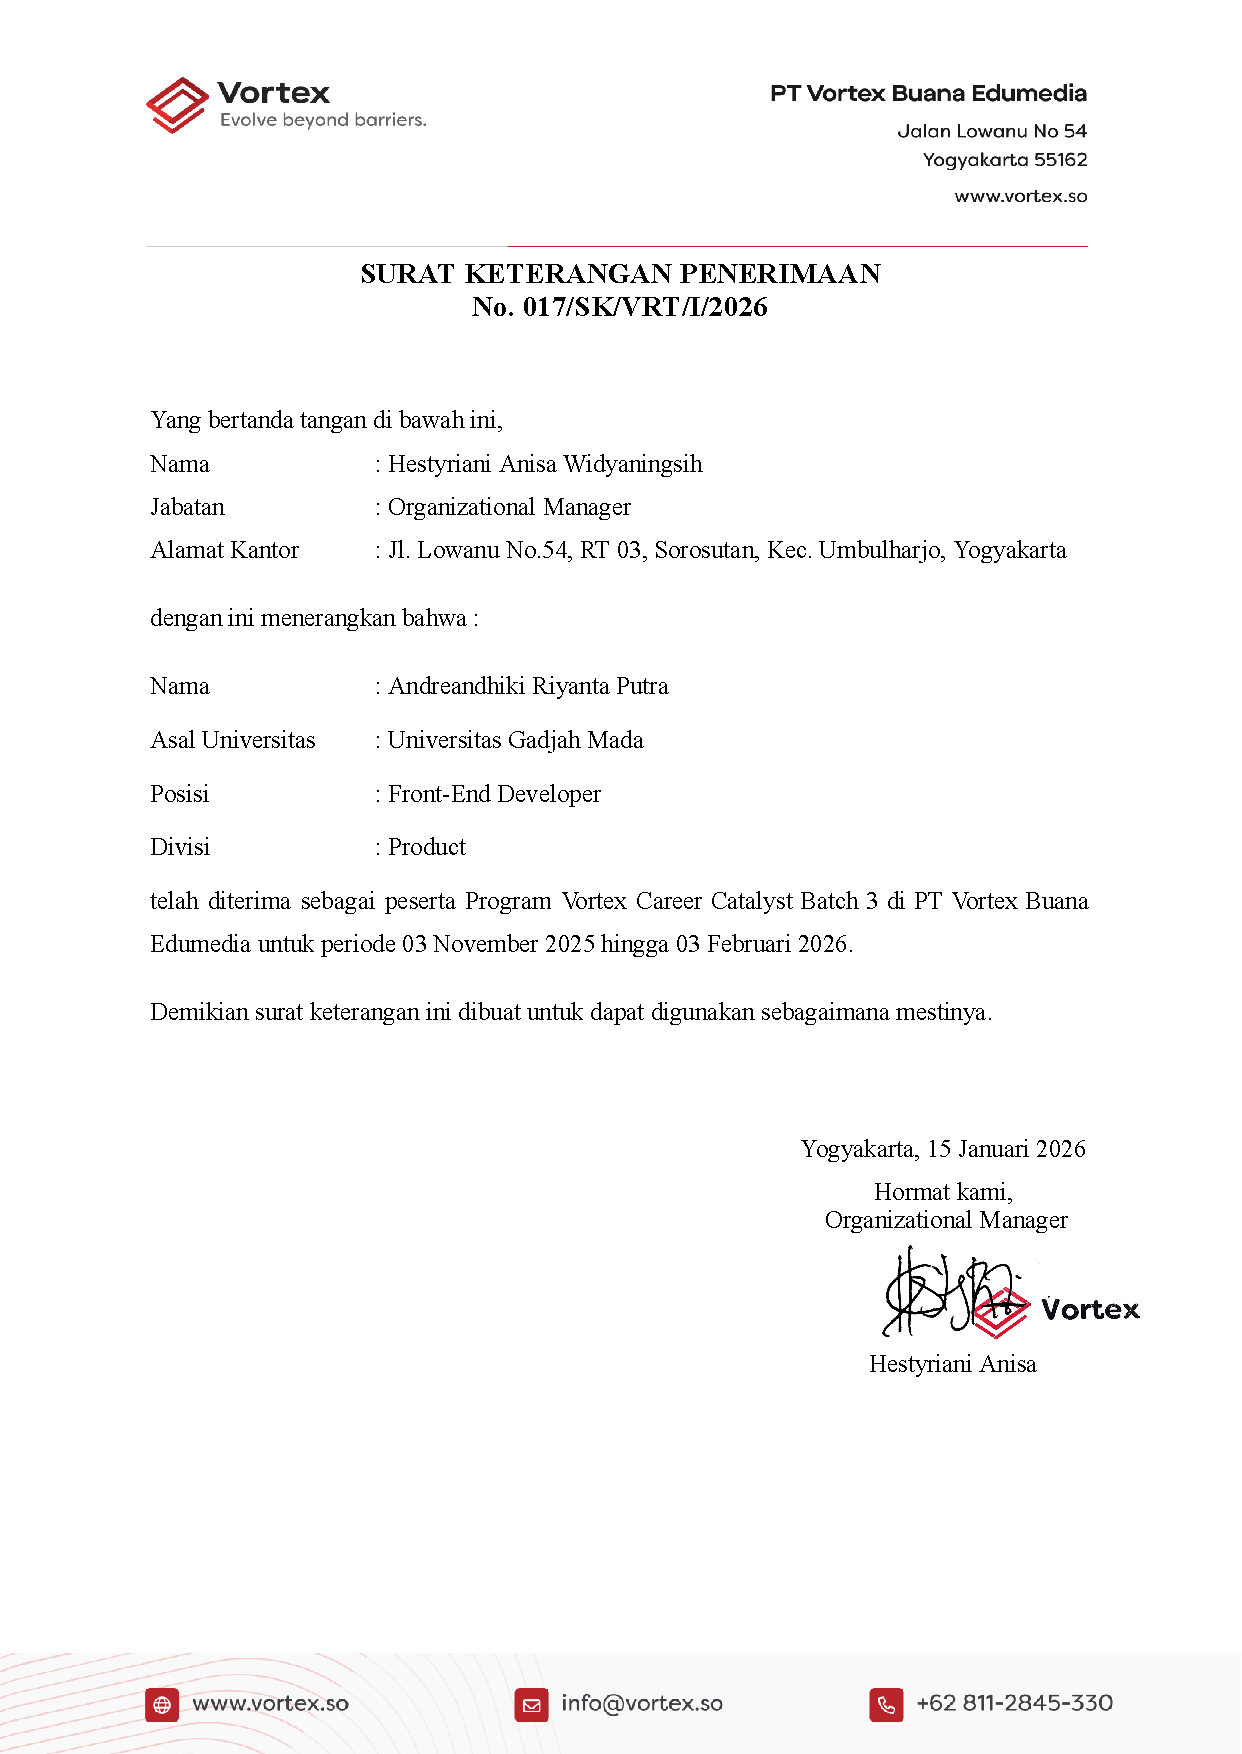
\includegraphics[width=\textwidth,height=0.72\textheight,keepaspectratio,page=1]{assets/LOA.pdf}
    \caption{Letter of Acceptance (halaman pertama)}
    \label{fig:lampiran_loa}
\end{figure}